\chapter{Teoria Estrutural}

\section{OS PRIMEIROS TEMPOS DA QUÍMICA ORGÂNICA}

Os povos pré-históricos conheciam as propriedades de alguns compostos orgânicos, sendo capazes de executar algumas reações envolvendo estes compostos. Os antigos egípcios, fenícios e romanos empregavam alguns corantes que eram compostos químicos em estado puro: índigo, alizarina e a lendária púrpura de Tiro. Os primeiros dois eram isolados de plantas e o último, obtido em pequenas quantidades a partir de uma espécie rara de moluscos.

A conversão de gordura animal em sabão, por tratamento com lixívia, é conhecida desde tempos antigos. Somente em 1948 os químicos orgânicos foram capazes de sintetizar produtos (detergentes) que podiam competir comercialmente com sabão. 

A fermentação de amido e açúcares para produção de álcool é conhecida desde os tempos pré-históricos e é usada, atualmente, quase sem modificações. 

A química orgânica, como a conhecemos hoje, teve seus começos no fim do século XVIII, quando um grande esforço foi iniciado para isolar compostos orgânicos puros que pudessem ser usados em substituição aos extratos. Entre 1769 e 1786, o alemão Scheele, que trabalhava na Suécia como boticário, isolou um certo número de compostos orgânicos de fontes naturais e estudou sua química. 

Em 1784, Lavoisier imaginou um método (discutido na Seção 2.2) para a queima de um composto orgânico e análise dos produtos de combustão. Embora fosse um processo de pouca precisão permitiu a Lavoisier inferir que a grande maioria dos compostos orgânicos era constituída de várias combinações dos elementos C, H, O e N. 

Em 1807, o químico sueco Berzelius foi o primeiro a usar o termo \textit{composto orgânico} para descrever substâncias extraídas de matéria viva, isto é, de \textit{sistemas organizados}. Berzelius e outros químicos de seu tempo acreditavam que compostos orgânicos possuíam uma "força vital", além dos elementos químicos que os compunham, e que seria tão impossível sintetizar um composto orgânico a partir de seus elementos, quanto converter a matéria inorgânica em uma criatura viva. Entretanto, a popularidade da teoria da "força vital" foi diminuindo, na medida em que as evidências analíticas iam se acumulando e mostrando que as leis usuais válidas para os materiais inorgânicos, tais como a lei das proporções múltiplas, funcionavam, também, para os compostos orgânicos. A teoria da `força vital` sofreu um severo golpe em 1828, quando Wölher descobriu que a evaporação de uma solução aquosa do sal inorgânico \textit{cianato de amônio} produzia \textit{uréia}, idêntica ao produto natural. Era a síntese de um composto orgânico típico, a partir de um composto inorgânico típico, sem a interferência de um organismo vivo que lhe comunicasse a "força vital". 

Em 1837, Liebig escreveu: "A extraordinária, e de algum modo inexplicável, produção da uréia sem a assistência das funções vitais, pela qual somos reconhecidos a Wöhler, deve ser considerada como uma das descobertas que marcam o início de uma nova era da ciência". No ano seguinte, Wöhler e Liebig, em um trabalho sobre o ácido lírico, afirmaram que todos os compostos seriam passíveis de preparação: "A filosofia da química chegará à conclusão de que a produção de todos os compostos orgânicos, desde que não façam parte de um organismo, deve ser vista não somente como provável, mas como certa." 

Melhores métodos de análise foram desenvolvidos, entre 1811 e 1831, principalmente por Gay-Lussac, Thénard e Dumas em Paris; Berzelius em Estocolmo e Liebig, em Giessen, na Alemanha. Os químicos aprenderam a determinar os elementos existentes nos compostos e suas proporções. Os métodos analíticos e sua aplicações são discutidos na Seção 2.2. 

Nos meados do século XIX, os métodos analíticos para a determinação dos elementos e radicais presentes em um composto orgânico e os, métodos sintéticos para a preparação de um composto, a partir de materiais mais simples, já estavam razoavelmente bem desenvolvidos, mas havia um aspecto da química orgânica que resistia aos esforços dos cientistas. Referimo-nos às \textit{estruturas} dos compostos orgânicos. Sabia-se, por exemplo, que álcool etílico e éter dimetílico têm a mesma fórmula (\ch{C2H60}), mas o primeiro é um componente das bebidas alcoólicas, enquanto o outro é um gás. Uma vez que estes dois compostos têm o mesmo tipo de átomos, a diferença entre eles, e entre muito outros grupos de compostos, era claramente devida à maneira pela qual os átomos estavam ligados, isto é, às estruturas das moléculas. O dilema pode ser melhor apreciado se dermos uma olhada nas estruturas corretas dos dois compostos. 

\begin{tightcenter}
    \chemnameinit{}
    \chemname{\chemname{\setchemfig{atom sep=2em}\chemfig[][]{H-C(-[2]H)(-[6]H)-C(-[2]H)(-[6]H)-O-H}}{\footnotesize{Álcool etílico}}}{\footnotesize{\ch{C2H6O}}}
    \qquad\qquad
    \chemnameinit{}
    \chemname{\chemname{\setchemfig{atom sep=2em}\chemfig[][]{H-C(-[2]H)(-[6]H)-O-C(-[2]H)(-[6]H)-H}}{\footnotesize{Éter dimetílico}}}{\footnotesize{\ch{C2H6O}}}
\end{tightcenter}

Os químicos, naquele tempo, enfrentavam um problema extremamente difícil. Gosta-riam de entender as estruturas das moléculas orgânicas, mas a única maneira de que dispunham para investigá-las eram reações químicas que causavam mudanças desconhecidas nas estruturas. Os caminhos que então foram tentados eram realmente complicados. Muito es-forço foi efetuado por alguns brilhantes cientistas: Frankland, em Manchester, Berzelius, Dumas e muitos outros para que se chegasse a uma melhor compreensão da estrutura molecular. Finalmente, em 1858, dois cientistas, Kekulé, em Heidelberg, e Couper, na Sorbonne, em Paris, independentemente introduziram as regras gerais das ligações de valência e a representação pictórica das moléculas como grupos de átomos ligados entre si. Eles também especificaram as regras que regem estas ligações, as quais são discutidas na Seção 2.3. 

\section{ANÁLISE QUÍMICA E FORMAS MOLECULARES}

O método da combustão, desenvolvido por Lavoisier, era capaz de dizer se carbono e hidrogênio estavam presentes em determinada substância e de dar uma idéia aproximada da quantidade de cada, mas não era suficientemente preciso para permitir estudos detalhados em compostos orgânicos. Um método de controle da combustão foi desenvolvido por Liebig, em 1831. Ele fez uso do fato, já então conhecido, de que vapores orgânicos são queimados, lenta e completamente, quando em contato com o óxido de cobre aquecido ao rubro, como ilustram as equações abaixo: 

\begin{tightcenter}
    \ch{CH4 + 4 CuO -> CO2 + 2 H2O + 4 Cu}
    
    \ch{C2H6O + 6 CuO -> 2 CO2 + 3 H2O + 6 Cu}
\end{tightcenter}

Por este método os químicos podiam determinar acuradamente a percentagem de cada elemento presente em um composto orgânico. 

\par\bigskip
\begin{leftbar}[cut=false]
\footnotesize
\noindent MATÉRIA OPCIONAL

\noindent \textit{Método de Liebig}. A Figura \ref{figurar_2_1} mostra em diagrama a aparelhagem usada para a combustão pelo mé-todo de Liebig. A amostra a ser queimada é vaporizada e o vapor misturado com oxigênio passa por um tubo carregado com óxido de cobre aquecido. O material orgânico é oxidado pelo óxido de cobre. O fluxo de oxigênio oxida novamente o cobre a óxido de cobre, carrega o dióxido de carbono e a água formados e passa por um tubo contendo um agente secante (usualmente perclorato de magnésio) e por um tubo contendo cal sodada. Na amostra inicial, o tubo de secagem e o tubo contendo cal sodada são pesados antes da combustão. Durante a combustão, quando o fluxo de oxigênio passa pelo tubo de secagem, a água fica retida e quando passapelo tubo contendo cal sodada, o dióxido de carbono é absorvido e transformado em carbonato. Após o término da combustão, os tubos de absorção são pesa-dos novamente. Obtém-se a quantidade de água formada na reação de combustão do aumento em peso do tubo de secagem. O aumento em peso do tubo contendo cal sodada fornece, do mesmo modo. a quantidade de dióxido de carbono formada.

\begin{figure}[H]
    \centering
    \captionsetup{width=0.93\linewidth}
    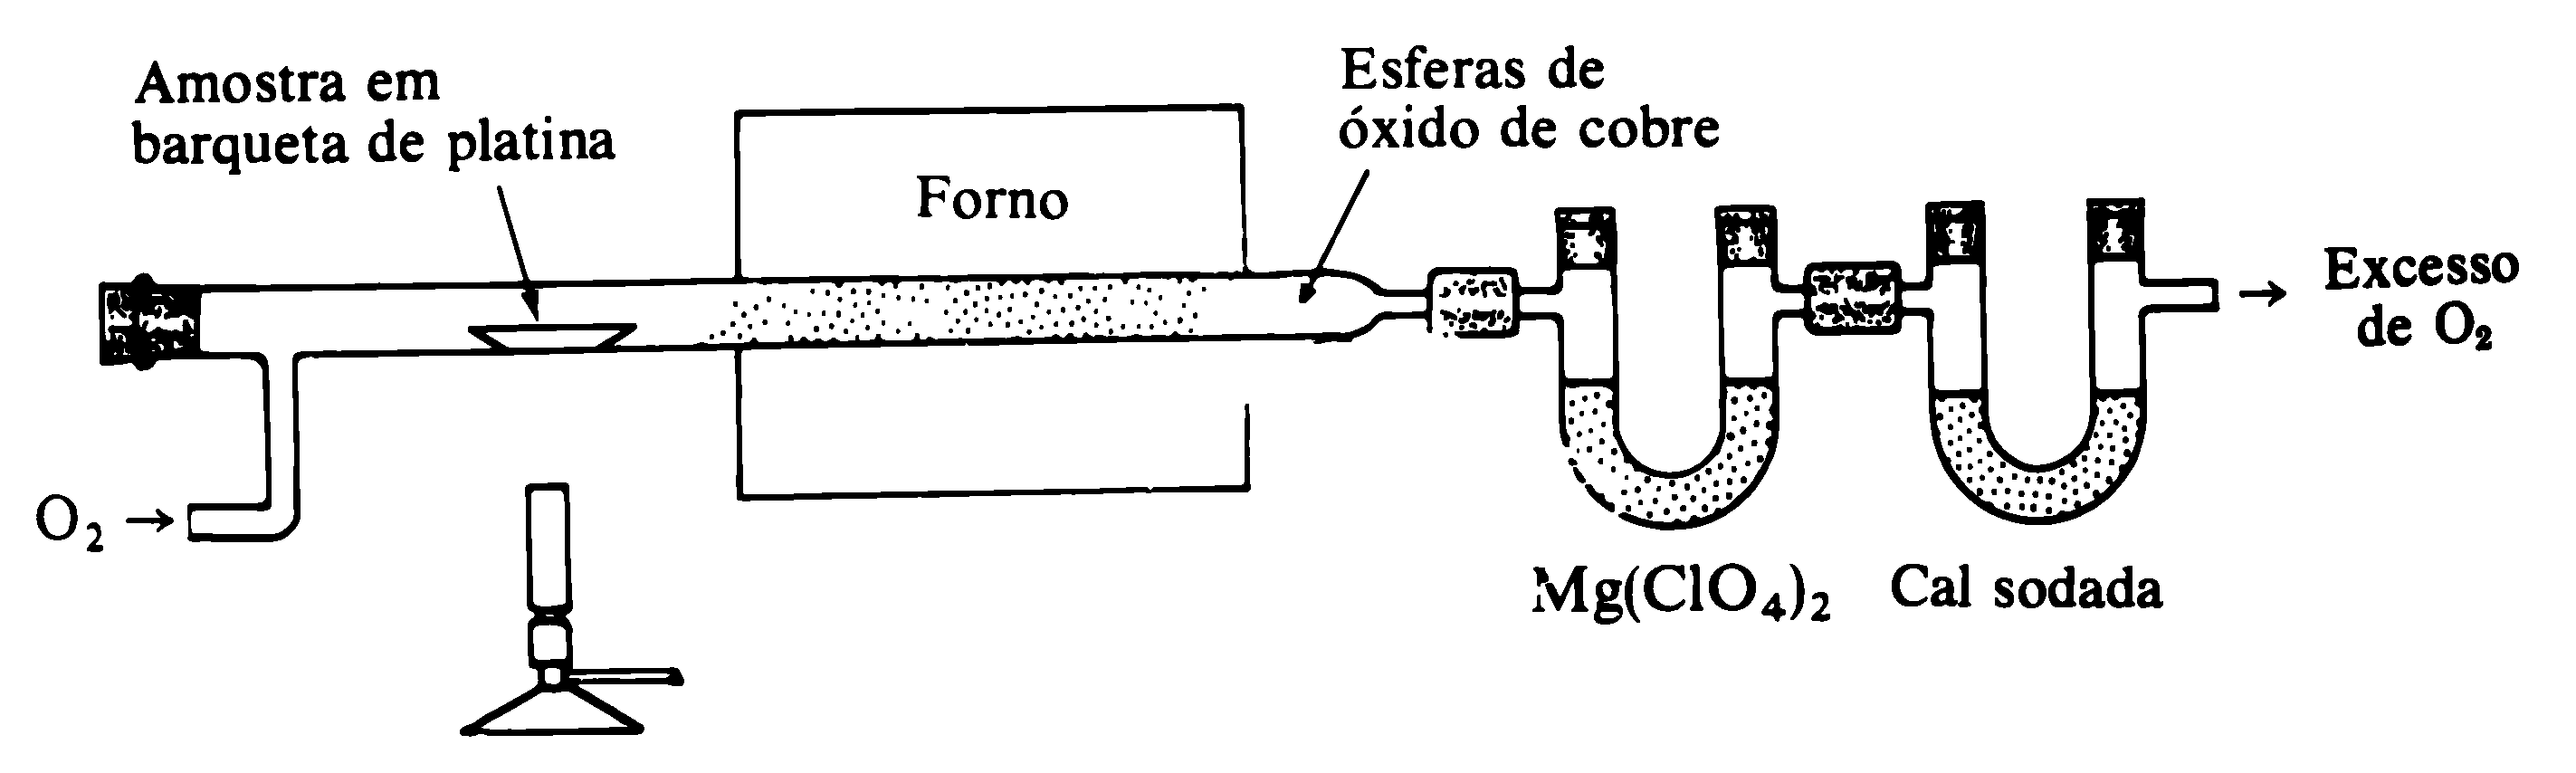
\includegraphics[scale=0.3]{content/images/Figura_2_1.pdf}
    \caption{Representação esquemática da aparelhagem usada para a analise de carbono e hidrogênio.}
    \label{figurar_2_1}
\end{figure}

Conhecendo as quantidades de dióxido de carbono e água produzidas no processo de combustão e a quantidade inicial de matéria orgânica queimada, pode-se calcular a percentagem de carbono e hidrogênio existentes na amostra original. O seguinte exemplo mostra o procedimento adequado. Usando os pesos atômicos H = 1,008, C = 12,01 e O = 16,000, o peso de hidrogênio na amostra é igual ao peso de água produzida vezes a fração de hidrogênio contida na água e o peso de carbono, o peso de dióxido de carbono produzido vezes a fração de carbono contida no dióxido de carbono.

\begin{tightcenter}
    \footnotesize
    g H = g \ch{H2O} $\times$ $\dfrac{2,016}{18,016}$ $\dfrac{\text{g H}}{\text{g \ch{H2O}}}$
    
    \% H = $\dfrac{\text{g H}}{\text{g Amostra}}$ $\times$ 100
    
    g C = g \ch{CO2} $\times$ $\dfrac{12,01}{44,01}$ $\dfrac{\text{g C}}{\text{g \ch{CO2}}}$
    
    \% C = $\dfrac{\text{g C}}{\text{g Amostra}}$ $\times$ 100
\end{tightcenter}

A análise não fornece diretamente a percentagem de oxigênio no composto. Pode-se, entretanto, supor que a percentagem da amostra que não seja carbono ou hidrogênio, e que se sabe não ser outro elemento (de testes preliminares), seja oxigênio, que é, assim, obtido por diferença. 
\end{leftbar}

\par\bigskip
\noindent\emph{No tempo de Liebig, os químicos orgânicos faziam suas próprias análises por combustão e era muito importante, para eles, entender os detalhes experimentais da combustão, pois a precisão obtida na análise dependia dos cuidados tomados durante a experiência. Hoje, o químico orgânico dificilmente faz as análises de que necessita, pois a área é controlada por um grupo de especialistas. Dada a amostra de um composto, eles darão ao químico orgânico a percentagem de cada elemento na amostra. O que é mais importante para o químico médio é que seja capaz de, urna vez conhecidas as percentagens dos elementos presentes, deduzir a fórmula para o composto em estudo. Deve ficar bem claro que a análise determina a percentagem de elementos na amostra. Se o composto não está puro, não serão obtidos bons resultados. Por outro lado, uma boa análise é evidência da pureza do composto.}
\par\bigskip

Como calculamos a fórmula de um composto, uma vez que a composição percentual é fornecida? Como um exemplo, seja a análise por combustão do éter metílico (um gás). Suponhamos que os seguintes valores fossem encontrados:

\begin{tightcenter}
53,24\% de carbono

13,05\% de hidrogênio
\end{tightcenter}

Testes qualitativos mostraram a ausência de outros elementos e, já que a percentagem total não atinge 100\%, a diferença deve ser devida ao oxigênio: 

\begin{tightcenter}
34,71\% de oxigênio 
\end{tightcenter}

Uma amostra de 100 g do composto, por exemplo, conteria 52,4 g de carbono, 13,05 g de hidrogênio e 34,71 g de oxigênio. Usando os números relativos em gramas destes elementos, queremos achar os números relativos em moles. Usando os pesos atômicos já fornecidos teremos em 100 g do composto:

\begin{tightcenter}
52,24/12,01 = 4,36 moles de carbono 

13,05/1,008 = 12,93 moles de hidrogênio 

34,71/16,00 = 2,16 moles de oxigênio 
\end{tightcenter}

Nossa tentativa inicial dá a fórmula C$_{4,36}$H$_{12,93}$O$_{2,16}$. Esta fórmula nos dá as razões corretas dos elementos. É evidente que a molécula contém menos átomos de oxigênio do que de carbono e hidrogênio. Como os átomos ocorrem apenas em números inteiros, então a molécula deve conter pelo menos um átomo de oxigênio, embora possa conter dois, três ou mesmo algum número maior. Se tomarmos os subscritos da fórmula e os dividirmos pelo menor deles (2,16) obteremos as razões corretas entre os elementos, na base da presença de um único átomo de oxigênio. A fórmula que obteremos é C$_{2,02}$H$_{5,98}$O. Existe sempre um erro experimental na análise (menor do que 0,3\%, se a análise for bem feita), e a fórmula que obtivemos, embora não tivesse números inteiros, pode ser tomada como sendo \ch{C2H6O}. Esta fórmula é chamada a \textit{fórmula empírica} do composto. É a fórmula, com a razão correta dos elementos, descrita pelo \textit{conjunto dos menores números inteiros}. A fórmula verdadeira poderia ser um múltiplo da fórmula que obtivemos. Por exemplo \ch{C4H12O2}, que contém exatamente a mesma razão elementar. Poderia ser, também, \ch{C6H18O3}, ou outro qualquer múltiplo da fórmula empírica. Para saber qual destas possibilidades representa a verdadeira \textit{fórmula molecular} do composto é preciso conhecer o peso molecular. Para um gás, o peso molecular pode ser obtido de medidas de pressão, volume e temperatura; para um líquido ou sólido, a partir do abaixamento do ponto de fusão de um solvente apropriado, ou, ainda, de várias outras maneiras. Digamos que para nosso composto, que é um gás, o peso de uma amostra de volume, pressão e temperatura conhecidos indica o peso molecular de 44,5. Para a fórmula empírica \ch{C2H6O} o peso molecular seria 46,1 ou um múltiplo deste número. Como o peso molecular experimental é mais próximo de 46,1 do que de qualquer um de seus múltiplos, podemos garantir que a fórmula molecular do composto é \ch{C2H6O}.

A importância de serem obtidas análises acuradas pode ser medida pelo exemplo seguinte. O ciclo-hexano tem a fórmula molecular \ch{C6H12}, enquanto que o composto chamado ciclo-hexeno, que possui propriedades diferentes, tem fórmula molecular \ch{C6H10}. A percentagem dos dois elementos presentes nestes compostos é, para \ch{C6H12}, de 85,6\% de carbono e 14,4\% de hidrogênio e, para \ch{C6H10}, de 87,7\% de carbono e 12,3\% de hidrogênio. O método analítico desenvolvido por Liebig tornou possível uma precisão de 0,3\% por elemento. Assim, o método de Liebig é capaz de distinguir entre os dois compostos mencionados. 

A desvantagem do método de Liebig, tal como era usado, é que requer uma quantidade que vai de 0,5 a 1,0 g de material para uma análise. O isolamento de um composto orgânico da natureza em forma pura é, frequentemente, muito difícil e muitos dos compostos que têm sido estudados nos últimos anos têm sido obtidos em quantidades muito pequenas. Um processo de microanálise foi introduzido por Pregl, em 1911, utilizando o método básico de Liebig, mas melhorando todos os instrumentos e acessórios envolvidos, especialmente a sensibilidade da balança usada para as pesagens. Pregl foi capaz de desenvolver o método de forma a que a análise fosse possível com 3 a 4 mg do material e recebeu o Prêmio Nobel por este trabalho.

\par\bigskip
\noindent\emph{Embora as fórmulas moleculares sejam, ainda hoje, determinadas pelo método de Pregl, outro método para efetuar esta determinação faz uso de um instrumento chamado espectrômetro de massas. Este aparelho bombardeia moléculas em fase gasosa com um feixe de elétrons. íons positivos, correspondendo à molécula original menos um elétron e aos diversos fragmentos moleculares, são formados e separados de acordo com a sua massa. Das massas destes íons é possível deduzir a fórmula molecular exata. O alto custo dos espectrômetros de massas (US\$30.000,00 a US\$100.000,00) temi evitado que este método seja mais difundido, mas isto ocorrerá certamente no futuro. O espectrômetro de massas será discutido com mais detalhes no Capítulo 32.}
\par\bigskip

\section{A TEORIA ESTRUTURAL DE KEKULÉ}

No campo da química inorgânica, uma vez conhecida a fórmula da substância, frequentemente a fórmula estrutural da molécula pode ser escrita sem problemas. Por exemplo. só existe um composto com a fórmula molecular \ch{Na2SO4}. O mesmo não acontece na química orgânica. Dois compostos, por exemplo, têm a fórmula molecular \ch{C4H10} e 14 compostos têm a fórmula molecular \ch{C5H12O}. Cada um destes 14 compostos têm propriedades físicas diferentes, tais como ponto de fusão e solubilidade e, consequentemente, correspondem a diferentes moléculas. Uma vez que esses compostos têm a mesma fórmula, deve haver algo diferente entre eles, isto é, os átomos devem estar ligados entre si de maneiras diferentes, de modo que a diferentes arranjos corresponderão diferentes compostos. A importância de entender como os átomos se ligam entre si para formar moléculas já era compreendida pelos cientistas nos começos do século XIX, mas os químicos do tempo não tinham como resolver o problema. A solução foi produzida independentemente por Kekulé e Cooper, em 1858. Estes cientistas postularam que o carbono teria a mesma valência 4 em moléculas orgânicas complicadas que têm nas substancias simples tais como tetracloreto de carbono (\ch{CCl4}) e dióxido de carbono (\ch{CO2}). O hidrogênio e o cloro têm valência 1, o oxigênio 2 e o nitrogênio trivalente 3. O carbono poderia ligar-se, então, a quatro átomos de cloro para formar metano (\ch{CH4}) ou a quatro átomos de cloro para formar tetracloreto de carbono. Usando essas valências, poderíamos escrever as fórmulas abaixo para dióxido de carbono, cianeto de hidrogênio (ácido cianídrico), metil-amina e etano:

\begin{tightcenter}
    \chemnameinit{}
    \chemname{\setchemfig{atom sep=2em}\chemfig[][]{Cl-C(-[2]Cl)(-[6]Cl)-Cl}}{\footnotesize{Tetracloreto de carbono}}
    \qquad\qquad\qquad
    \chemnameinit{}
    \chemname{\setchemfig{atom sep=2em}\chemfig[][]{O=C=O}}{\footnotesize{Dióxido de carbono}}
    \qquad\qquad\qquad
    \chemnameinit{}
    \chemname{\setchemfig{atom sep=2em}\chemfig[][]{H-C~N}}{\footnotesize{Cianeto de hidrogênio}}
\end{tightcenter}

\begin{tightcenter}
    \chemnameinit{}
    \chemname{\setchemfig{atom sep=2em}\chemfig[][]{H-C(-[2]H)(-[6]H)-H}}{\footnotesize{Metano}}
    \qquad\qquad\qquad
    \chemnameinit{}
    \chemname{\setchemfig{atom sep=2em}\chemfig[][]{H-C(-[2]H)(-[6]H)-C(-[2]H)(-[6]H)-H}}{\footnotesize{Etano}}
    \qquad\qquad\qquad
    \chemnameinit{}
    \chemname{\setchemfig{atom sep=2em}\chemfig[][]{H-C(-[2]H)(-[6]H)-N(-[2]H)-H}}{\footnotesize{Metil-amina}}
\end{tightcenter}
 
Quando duas moléculas diferentes têm a mesma fórmula molecular são chamadas de \textit{isômeros}. Álcool etílico e éter dimetílico são isômeros com fórmula molecular \ch{C2H6O}: 

\begin{tightcenter}
    \chemnameinit{}
    \chemname{\setchemfig{atom sep=2em}\chemfig[][]{H-C(-[2]H)(-[6]H)-C(-[2]H)(-[6]H)-OH} = \ch{CH3CH2OH}}{\footnotesize{Álcool etílico}}
    \qquad\qquad\qquad
    \chemnameinit{}
    \chemname{\setchemfig{atom sep=2em}\chemfig[][]{H-C(-[2]H)(-[6]H)-O-C(-[2]H)(-[6]H)-H } = \ch{CH3OCH3}}{\footnotesize{Éter dimetílico}}
\end{tightcenter}

Deve ficar bem claro ao leitor que, segundo as regras de valência de Kekulé, estas são as duas únicas maneiras em que estes átomos podem ser arranjados. 

Como dizer experimentalmente a qual estrutura corresponde determinado composto é um problema com o qual nos preocuparemos nos próximos capítulos. 

\section{A LIGAÇÃO COVALENTE}

Kekulé usava uma linha simples para representar a ligação química entre dois átomos, mas não estava clara qual a natureza física desta ligação química. O desenvolvimento do que consideramos, atualmente, uma teoria razoável sobre a natureza das ligações químicas e as estruturas das moléculas orgânicas só foi possível após a descoberta do elétron, em 1897, por J. J. Thompson, e a posterior descrição devida a Lorde Rutherford, em 1911, de um átomo como sendo um sistema formado por pequeno núcleo positivo cercado por elétrons a uma distância relativamente grande. 

Em 1916, Lewis em Berkeley e W. Kossel, em Munique, utilizaram-se do modelo de Rutherford para explicar muitas das propriedades químicas dos átomos e de seus íons. Lewis desenvolveu o modelo, de modo a incluir as ligações covalentes de maneira a permitir a expressão das primeiras idéias sobre a teoria estrutural em termos das partículas fundamentais, núcleo e elétron. A teoria de Lewis é fundamental para o entendimento das estruturas de compostos e das propriedades químicas de moléculas orgânicas em termos clássicos e, graças à sua simplicidade, ainda hoje é largamente utilizada para descrições qualitativas de fenômenos da química orgânica. 

Desde os começos de sua ciência, os químicos orgânicos imaginaram teorias que pudessem explicar suas observações. Uma boa teoria explica todos os fatos nos quais é baseada e pode ser utilizada para a previsão de novos fatos que, por sua vez, podem ser verificados pela experiência. Por causa do desconhecimento, durante o século XIX, da natureza do átomo, as teorias sobre as estruturas e reações de moléculas orgânicas não se desenvolveram com rapidez para ser de valor na predição de novos fatos. Ao contrário, os químicos estavam principalmente preocupados com a explicação de fatos já conhecidos experimentalmente. No entanto, as idéias de Kekulé e de seus contemporâneos eram essencialmente corretas, e os modernos químicos têm a maior admiração pelos cientistas que fizeram o extraordinário trabalho de deduzir as estruturas das moléculas muito antes que os fatos correspondentes aos átomos fossem compreendidos. 

Todavia muitos dos problemas estruturais mais complicados não foram entendidos até cerca de 1930, quando a teoria quantomecânica foi desenvolvida. Não seguiremos, neste capítulo, o desenvolvimento histórico da teoria estrutural por ser um caminho extremamente difícil e trabalhoso, embora de proveito intelectual. Utilizando-nos das idéias essenciais da teoria estrutural, é possível deduzir praticamente todos os fatos relativos as estruturas das moléculas orgânicas nos quais estaremos interessados. Este modo de abordar o problema é vantajoso, no momento, porque liberta o estudante da necessidade de tratar uma quantidade enorme de fatos experimentais e mostra como todos os fatos se tornam evidentes, desde que a teoria seja compreendida. Deve ser enfatizado, entretanto, que, historicamente, tudo se passou de maneira diferente. 

Podem-se reconhecer três tipos de ligação: iônica, metálica e covalente. A \textit{ligação iônica} (\textit{e.g.} \ch{NaCl}) foi muito bem descrita por Lewis e também por Kossel. Na verdade, não se trata de uma ligação, na acepção do termo, mas uma atração eletrostática sem direção preferencial. A \textit{ligação metálica} é característica dos metais em fase sólida e líquida e não nos interessa discuti-la presentemente. Moléculas orgânicas são formadas por átomos em \textit{ligação covalente} e tais ligações formam a base da química orgânica. A teoria de Lewis foi a primeira etapa na compreensão da ligação covalente e, qualitativamente, as idéias em que se baseava estavam essencialmente corretas, já que explicavam a maior parte dos fenômenos. A ligação covalente existe entre pares, de átomos que tendem a completar suas camadas eletrônicas por partilha de elétrons e é, geralmente, mais forte quando um ou ambos os átomos pertencem a um dos grupos centrais da tabela periódica. Um átomo de carbono dificilmente forma ligações iônicas, pois, para tal, seria necessária uma carga +4 ou -4 concentrada em um átomo relativamente pequeno — uma situação altamente desfavorável energeticamente.

\begin{tightcenter}
    C: 1s$^2$2s$^2$2p$^2$ \ch{->} 1s$^2$2s$^0$p$^0$ ou C$^{4-}$: 1s$^2$2s$^2$2p$^6$
\end{tightcenter}

Em vez de perder ou ganhar elétrons de forma definitiva para formar íons, um átomo de carbono tende a partilhar elétrons em ligações covalentes. Muitas moléculas inorgânicas são igualmente formadas por ligações covalentes, como \textit{e.g.}, \ch{N2}, \ch{AsCl3} e \ch{H2O}. 

\par\bigskip
\noindent REVISÃO DAS ESTRUTURAS DE LEWIS. \textit{Será necessário ao leitor recordar o que são estruturas de Lewis, como se representam e o que é} carga formal. \textit{Os próximos parágrafos o ajudarão nisto.} 

\emph{Lewis notou que os sistemas eletrônicos dos gases nobres podem ser considerados como sendo compostos de camadas de elétrons, contendo nas camadas eletrônicas exteriores, respectivamente, 2 elétrons (hélio), 8 elétrons (neônio), 8 elétrons (argônio) e assim por diante. Os gases nobres são muito estáveis e inertes quimicamente. Sistemas eletrônicos semelhantes apresentam, também, relativa estabilidade e inércia química. Temos, assim, F$^-$ com a configuração eletrônica do neônio e K$^+$ com a configuração do argônio. Metano, amoníaco, água e fluoreto de hidrogênio têm, também, 8 elétrons na camada exterior do elemento pesado (desde que contemos os elétrons partilhados) e 2 elétrons na camada eletrônica dos hidrogênios. Todas essas moléculas são eletronicamente análogas aos gases nobres e são substâncias covalentes muito estáveis. Suas estruturas podem ser representadas como se segue:}

\begin{tightcenter}
    \chemnameinit{}
    \chemname{\chemfig[][]{\lewis{0:2:4:6:,C}(-[2,0.4,,,draw=none]H)(-[4,0.4,,,draw=none]H)(-[6,0.4,,,draw=none]H)(-[0,0.4,,,draw=none]H)}}{\footnotesize{Methano}}
    \qquad    
    \chemnameinit{}
    \chemname{\chemfig[][]{\lewis{0:2:4:6:,N}(-[4,0.4,,,draw=none]H)(-[6,0.4,,,draw=none]H)(-[0,0.4,,,draw=none]H)}}{\footnotesize{Amoníaco}}
    \qquad    
    \chemnameinit{}
    \chemname{\chemfig[][]{\lewis{0:2:4:6:,O}(-[4,0.4,,,draw=none]H)(-[6,0.4,,,draw=none]H)}}{\footnotesize{Água}}
    \qquad\qquad\qquad    
    \chemnameinit{}
    \chemname{\chemfig[][]{\lewis{0:2:4:6:,F}(-[4,0.4,,,draw=none]H)}}{\footnotesize{Fluoreto de hidrogênio}}
    \qquad\qquad\qquad    
    \chemnameinit{}
    \chemname{\chemfig[][]{\lewis{0:,He}}}{\footnotesize{Hélio}}
    \qquad    
    \chemnameinit{}
    \chemname{\chemfig[][]{\lewis{0:2:4:6:,Ne}}}{\footnotesize{Neônio}}
\end{tightcenter}

\emph{Para determinar a carga formal de um átomo, contam-se todos os elétrons que, na formula de Lewis, pertencem exclusivamente ao átomo, mais a metade dos elétrons partilhados em ligações covalentes. Se este número é igual ao número de elétrons de valência do átomo livre, a carga formal do átomo na fórmula de Lewis é zero. Se o número de elétrons excede o número de elétrons de valência do átomo livre por 1, 2, 3, ..., então a carga formal do átomo na estrutura de Lewis é -1, —2, —3, .... Se, por outro lado, o numero de elétrons é menor do que o número de elétrons de valência do átomo livre por 1, 2, 3, ..., então a carga formal do átomo na estrutura de Lewis é +1, +2, +3, ....}

\emph{Alguns exemplos do cálculo de cargas formais podem ilustrar melhor o exposto. Na molécula de metano cada átomo tem uma carga formal zero, uma vez que a metade do número de elétrons em ligação covalente é igual ao número de elétrons de valência do átomo de carbono livre (carga formal = 4 - 4 = O), o mesmo acontecendo para os hidrogênios (carga formal = 1 - 1 = O). Pode ser igualmente verificado que todos os átomos em \ch{NH3}, \ch{H2O} e \ch{HF} têm carga formal zero.}

\emph{Examine, agora, as estruturas abaixo:}

\begin{tightcenter}
    \chemnameinit{}
    \chemname{\chemfig[][]{\lewis{0:2:4:6:,\chemabove{N}{\hspace{+5mm}\scriptstyle +}}(-[2,0.4,,,draw=none]H)(-[4,0.4,,,draw=none]H)(-[6,0.4,,,draw=none]H)(-[0,0.4,,,draw=none]H)}}{\footnotesize{Íon amônio}}
    \qquad
    \chemnameinit{}
    \qquad 
    \chemfig[][]{\lewis{0:4:,C}(-[4,0.4,,,draw=none]H)}
\end{tightcenter}


\emph{Note que todos os átomos têm 8 elétrons na camada de valência (exceto os hidrogênios que têm 2). O íon amônio tem 1/2 $\times$ 8 = 4 elétrons que pertencem ao nitrogênio. Como o nitrogênio isolado tem 5 elétrons, há uma carga formal +1 no nitrogênio do íon amônio.}

\emph{Na molécula \ch{HCN}, o H tem uma carga formal zero (1 - 2/2), assim como o carbono (4 - 8/2) e o nitrogênio (5 - 2 - 6/2). No caso do \ch{CN-}, o nitrogênio tem formalmente 5 elétrons e carga formal zero, enquanto o carbono tem 5 elétrons e, portanto, carga formal -1.}

\par\bigskip
O leitor deve lembrar-se de que a descrição exata do átomo de hidrogênio pode ser obtida pela solução da equação de Schrödinger: 

\begin{equation}
    \setlength{\topsep}{.5ex}
    H\psi = E\psi
\end{equation}

\noindent onde existe um conjunto infinito de funções de onda psi ($\psi$) chamadas \textit{orbitais}. Cada orbital é uma função matemática que descreve uma distribuição possível do elétron no espaço. Cada um destes orbitais tem uma energia (\textit{E}) a ele associada. O elétron pode ocupar qualquer um destes orbitais e os átomos adquirem a energia correspondente. 

\par\bigskip
\noindent\emph{O resto desta seção e parte do material subsequente referir-se-á à solução da equação de Schrödinger. A matemática necessária para solucionar a equação é muito complicada e, neste texto, estaremos muito mais interessados em usar os resultados que podem ser obtidos do que nos detalhes de sua obtenção.}
\par\bigskip

A parte complicada da equação é \textbf{H}, o operador Hamiltoniano. (Um operador é um símbolo matemático que nos diz como manipular a quantidade que o segue.) Este operador contém as segundas derivadas de $\psi$ com respeito às coordenadas. Para resolver a equação, deve-se integrá-la. Infelizmente, isto só pode ser feito de maneira exata em alguns casos, tais como o do átomo de hidrogênio. Soluções aproximadas (com muitos algarismos significativos) já foram obtidas para átomos de baixo número atômico e para algumas moléculas pequenas. Mesmo o átomo de hélio já é muito complicado para que se possa obter, com as técnicas de hoje, uma solução exata, mas a energia pode ser calculada por métodos aproximados até 8 algarismos significativos. Não há dúvida nenhuma de que a equação é igual-mente válida para moléculas maiores, mas, para estes casos, mesmo os métodos aproximados de que dispomos são limitados, dada a complexidade matemática do problema. 

O sistema mais simples que contém uma ligação covalente normal (um par de elétrons) é a molécula de hidrogênio (\ch{H2}). Esta molécula vem sendo estudada teoricamente com cuidado. É mais complicada do que o átomo de hélio, embora se pareça muito com ele. Se chamarmos os dois núcleos de hidrogênio da molécula \ch{H2}, H$_A$ e H$_B$, podemos usar o orbital atômicos 1s do hidrogênio para cada um dos átomos ($\psi _A$ e $\psi _B$) e escrever um \textit{orbital molecular} $\psi _A + \psi _B$. No nosso caso, o orbital molecular é formado por uma combinação linear de orbitais atômicos. Do mesmo modo que um orbital atômico nos diz onde o elétron deve ser encontrado no espaço tridimensional ao redor do núcleo, um orbital molecular nos diz onde deve encontrar-se o elétron no espaço tridimensional da molécula. (Lembre-se de que o valor de $\psi ^2$ em qualquer ponto deste espaço é proporcional à densidade eletrônica,, isto é, à probabilidade de encontrar-se o elétron naquele ponto.) A forma do orbital molecular ou a função da probabilidade de encontrar-se um elétron no espaço tridimensional da molécula é, geralmente, muito mais complicada do que a de um orbital atômico. Como acontece com o átomo de hélio, quanto mais refinados os cálculos, melhor a concordância entre os valores experimentais e calculados para as distâncias de ligação e energias. A idéia de que os orbitais moleculares sejam formados por combinações de orbitais atômicos é muito importante. Ela nos permite interpretar a estrutura das moléculas em termos das estruturas dos átomos, os quais conhecemos relativamente bem, graças à analogia que podemos fazer com o caso do átomo de hidrogênio, no qual a equação de Schrödinger pode ser resolvida exatamente. \textit{A matemática da formação de orbitais moleculares é de tal natureza que, em geral, se começamos com n orbitais atômicos e os combinamos, obteremos sempre n orbitais moleculares.} As energias dos n orbitais moleculares serão diferentes das energias dos orbitais atômicos dos quais foram formados. Alguns dos orbitais têm energia mais baixa e são chamados orbitais ligantes, enquanto outros têm energia mais alta e são chamados orbitais antiligantes. Pode acontecer que um, ou mais de um, dos orbitais moleculares tenha a mesma energia do que um dos orbitais atômicos e, neste caso, é chamado orbital não-ligante. Para a molécula de hidrogênio, a solução da equação de Schrödinger dá dois orbitais moleculares ($\psi$ e $\psi ^*$) que são combinações dos orbitais atômicos: 

\begin{equation}
    \setlength{\topsep}{.5ex}
    \psi = \psi _A + \psi _B
    \qquad e \qquad
    \psi ^* = \psi _A - \psi _B
\end{equation}

O primeiro dos orbitais ($\psi$) é um orbital ligante, enquanto o segundo ($\psi ^*$) é antiligante (veja Figura 2.2). Os orbitais moleculares são como os orbitais atômicos, no sentido de que são capazes de suportar no máximo dois elétrons e, assim mesmo, se tiverem spins opostos. É evidente que ambos os elétrons da molécula do hidrogênio ocuparão o orbital ligante (de menor energia) e, nestas circunstâncias, a energia do sistema será mínima quando a separação entre os dois núcleos for de 0,74 \AA ngstrom (\AA). Estes elétrons de ligação estão, portanto, numa situação de maior estabilidade do que estariam, se cada elétron estivesse em um átomo de hidrogênio isolado, e tendem a permanecer nesta situação, mantendo unidos os núcleos e formando uma ligação química. Mais precisamente, eles formam uma ligação com um comprimento de 0,74 \AA \enspace e com força de ligação correspondente à profundidade do poço de potencial no qual estão os elétrons. Por outro lado, elétrons colocados em orbitais antiligantes evitam a região do espaço entre os núcleos, tendendo, deste modo, a mantê-los separados. 

\begin{figure}[H]
    \centering
    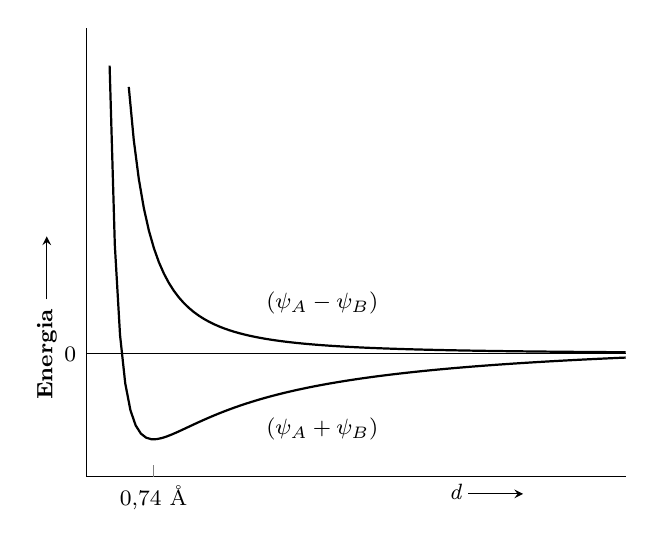
\begin{tikzpicture}[help lines/.style={thin,draw=black!50}]
        %\draw[help lines] (0,0) grid (15,12);
        \node (z) at (3,2.2) {\footnotesize{($\psi _A - \psi _B$)}};
        \node (y) at (3,0.6) {\footnotesize{$(\psi _A + \psi _B$)}};
        \node (x) at (4.7,-0.2) {\footnotesize{\textit{d}}};
        \draw [->,>=stealth] (4.85,-0.22) -- ++(0:0.7);
        \node (m) at (-0.2,1.55) {\footnotesize{0}};
        \node [rotate=90] (t) at (-0.5,1.55) {\footnotesize{\textbf{Energia}}};
        \draw [->,>=stealth] (t) -- ++(90:1.5);
        
        % Set horizontal range 
        \pgfmathsetmacro{\nx}{8}
        % Set vertical range 
        \pgfmathsetmacro{\ny}{2.5}
        
        \pgfmathsetmacro{\xmin}{2*(sqrt(\ny+1)-1)/\ny}
        \pgfmathsetmacro{\xmint}{2/sqrt(\ny)}
        \pgfmathsetmacro{\xminb}{4/\ny}
        \pgfmathsetmacro{\xmax}{2*\nx}
        
        \begin{axis}[xmin=0,xmax=\xmax,axis x line*=bottom,axis y line*=left,xtick=\empty,ytick=\empty,extra x ticks={2},extra x tick labels={\footnotesize{0,74 \AA}}]
            \addplot[thick,domain=\xmin:\xmax,samples=100]{1/x^2-1/x+0.05};
            %\addplot[domain=\xminb:\xmax,samples=100]{-1/x};
            \addplot[thick,domain=\xmint:\xmax,samples=100]{1/x^2};
            \addplot[no markers] coordinates {(0,0) (\xmax,0)};
        \end{axis}
    \end{tikzpicture}
    \caption{Energia de dois átomos de hidrogênio em função da distância (\textit{d}) entre os núcleos quando os elétrons ocupam orbitais ligantes é antiligantes.}
    \label{figura_2_2}
\end{figure}

\begin{figure}[H]
    \centering
    \adjustbox{margin=1em,width=\textwidth,set height=4cm,set depth=4cm,frame,center}{Dummy}
    \caption{Orbital de ligação da molécula do hidrogênio.}
    \label{fig2_3}
\end{figure}

Desde o tempo de Kekulé, os químicos orgânicos usam uma linha simples para representar uma ligação covalente e ainda hoje o fazem. Todavia, nossa compreensão do que a linha simples realmente representa alterou-se muito. graças ao nosso melhor conhecimento dos fenômenos que governam a ligação química. Vários outros modos de representação dos orbitais moleculares encontram-se na Figura \ref{fig2_3}. A maneira mais simples de representar os orbitais $1s$ é utilizando-se de círculos. Deve-se, entretanto, ter em mente que cada círculo representa na realidade uma esfera que contém uma boa parte, digamos 90\%, da densidade eletrônica do orbital em seu interior. A Figura ensombrecida representa a probabilidade de distribuição do elétron: quanto mais forte for a sombra, maior será a probabilidade de encontrar-se o elétron naquela posição. Um mapa de contorno de densidade eletrônica frequentemente é útil. A ligação existente na molécula \ch{H2} é uma ligação covalente típica, semelhante àquelas encontradas em moléculas orgânicas. Em uma molécula complicada é, geral-mente, uma boa aproximação da realidade considerarem-se os átomos ligados aos pares por ligações covalentes. 

Uma ligação covalente entre quaisquer dois átomos é descrita por uma função de onda que tem uma certa semelhança com a que usamos para a molécula de hidrogênio. Para uma molécula como \ch{HF}, a função de onda para o orbital ligante é tal que existe maior densidade eletrônica no átomo eletronegativo (flúor), como aliás seria de se esperar. A função de onda de ligação para \ch{HF} é $\psi = \psi$H$_{1s} + \lambda\psi$F$_{2p}$, onde lambda ($\lambda$) > 1, correspondendo a uma densidade eletrônica maior na parte F$_{2p}$ do orbital de ligação do que na parte H$_{1s}$. 

Por outro lado, o elétron no orbital antiligante gasta a maior parte de seu tempo perto do elemento eletropositivo. As densidades eletrônicas correspondentes aos orbitais ligante e antiligante da molécula do fluoreto de hidrogênio estão na Figura \ref{fig2_4}. (Os átomos de flúor têm muitos elétrons não-ligantes que não aparecem na Figura. Observe que o átomo de flúor usa um orbital $2p$ para formar a ligação.) Se os elétrons estão no orbital de ligação, tendem a concentrar-se entre os núcleos. O orbital de antiligação tem um nodo (superfície de densidade eletrônica zero) e os elétrons tendem a evitar esta região. 

\par\bigskip
\noindent\emph{O leitor pode muito bem perguntar: mas como o elétron é capaz de atravessar o nodo? A resposta mais direta é que os nodos são preditos na base de matemática não-relativística e os livros-texto geralmente esquecem-se de mencionar que, quando os efeitos da relatividade são levados em consideração, a superfície de densidade eletrônica "zero" tem uma densidade eletrônica finita (embora muito pequena). O nodo é, portanto, na realidade só uma aproximação e o elétron pode cruzá-lo sem problemas.}
\par\bigskip

O estado de mais baixa energia para a molécula é geralmente aquele que nos interessa mais e é chamado \textit{estado fundamental}. Se dermos energia à molécula (da maneira correta), é possível excitar-se um elétron de um orbital ligante a um orbital antiligante. Esta absorção de energia ocorre apenas em determinados comprimentos de onda (energias) que dependem das diferenças de energia entre o orbital ocupado pelo elétron no estado fundamental e nos diversos estados excitados. As excitações eletrônicas que ocorrem corresponderão ao espectro de absorção da molécula. Um \textit{espectro de absorção} é medido pela diferença de quantidade de radiação incidente em uma substância e a quantidade capaz de atravessá-la. Esta diferença é usada para excitar os átomos ou moléculas a estados de mais alta energia. Frequentemente o espectro de absorção de uma substância permite inferir-se muitas informações relevantes sobre a estrutura molecular; por isto voltaremos ao assunto em capítulos subsequentes. 

\begin{figure}[H]
    \centering
    \adjustbox{margin=1em,width=\textwidth,set height=4cm,set depth=4cm,frame,center}{Dummy}
    \caption{Orbitais ligantes e antiligantes do fluoreto do hidrogênio.}
    \label{fig2_4}
\end{figure}

A cor amarela que aparece em uma chama toda vez que nela colocamos um pouco de sódio é um exemplo familiar de \textit{espectro de emissão}. O sódio adquire energia térmica da chama e os seus elétrons são excitados a orbitais de mais alta energia. Quando os elétrons voltam aos níveis de mais baixa energia, luz de diversos comprimentos de onda é emitida, inclusive na região do visível, e, assim, podemos ver a cor amarela característica. O espectro de emissão é medido pela radiação fornecida quando os elétrons voltam dos estados excitados ao fundamental.

\section{ESTRUTURA DO METANO}

o metano é o constituinte principal do gás natural que usamos como combustível. Algumas vezes é chamado \textit{gás dos pântanos} porque é o produto da decomposição de vegetais em condições anaeróbicas. O metano tem fórmula \ch{CH4}, e é o \textit{hidrocarboneto} (molécula contendo apenas carbono e hidrogênio) mais simples. No século passado ficou estabelecido que esta molécula tem a forma de um tetraedro regular (Figura \ref{figura_2_5}) com hidrogênios nos quatro vértices e carbono no centro, sendo os ângulos \ch{HCH} de 109,5$\degree$. A prova desta estrutura residia no fato, que pode ser mostrado experimentalmente: os quatro hidrogênios são equivalentes. Assim, existe apenas um cloreto de metileno, \ch{CH_2Cl_2}. Uma vez que os quatro vértices de um tetraedro regular são equivalentes, não faz diferença qual grupo de dois hidrogênios é substituído por cloro, porque a mesma estrutura resultará sempre. Observe que, se a estrutura da molécula fosse a de um quadrado em um plano, por exemplo, os átomos de cloro poderiam estar em vértices adjacentes, ou não, e haveria assim dois compostos com estruturas diferentes e com a fórmula \ch{CH_2Cl_2} (Figura \ref{figura_2_6}).

\begin{figure}[H]
    \centering
    \begin{tikzpicture}[help lines/.style={thin,draw=black!50}] 
        % \draw[help lines] (0,0) grid (15,12);
        \path (0,0) node (m) {C} (2,0) node (x) {H};
        \node (z) at ($ (m) + (100:2) $) {H};
        \node (y) at ($ (m) + (310:2) $) {H};
        \node (w) at ($ (m) + (200:3) $) {H};
        \draw[thick] (m) -- (z);
        \draw[thick] (m) -- (x);
        \draw[thick] (m) -- (y);
        \draw[thick] (m) -- (w);
        \draw[dashed] (x) -- (y) -- (z) -- (x);
        \draw[dashed] (z) -- (w) -- (y) -- (z);
        \draw[dashed] (w) -- (x);
    \end{tikzpicture}
    \caption{Estrutura de tetraedro regular do metano (as linhas interrompidas são imaginarias e são incluídas apenas para facilitar a visualização do tetraedro.}
    \label{figura_2_5}
\end{figure}

\begin{figure}[H]
    \centering
    \begin{tikzpicture}[help lines/.style={thin,draw=black!50}] 
        % \draw[help lines] (0,0) grid (15,12);
        \path (0,0) node (m) {C};
        \node (z) at ($ (m) + (45:2) $) {H};
        \node (x) at ($ (m) + (155:3) $) {H};
        \node (w) at ($ (m) + (225:2) $) {Cl};
        \node (y) at ($ (m) + (334:3) $) {Cl};
        \draw[thick] (m) -- (z);
        \draw[thick] (m) -- (x);
        \draw[thick] (m) -- (y);
        \draw[thick] (m) -- (w);
        \draw[dashed] (z) -- (x) -- (w) -- (y) -- (z);
        % isômero
        \path (7,0) node (m2) {C};
        \node (z2) at ($ (m2) + (45:2) $) {H};
        \node (x2) at ($ (m2) + (155:3) $) {Cl};
        \node (w2) at ($ (m2) + (225:2) $) {H};
        \node (y2) at ($ (m2) + (334:3) $) {Cl};
        \draw[thick] (m2) -- (z2);
        \draw[thick] (m2) -- (x2);
        \draw[thick] (m2) -- (y2);
        \draw[thick] (m2) -- (w2);
        \draw[dashed] (z2) -- (x2) -- (w2) -- (y2) -- (z2);
    \end{tikzpicture}
    \caption{Isômeros que seriam possíveis se o cloreto de metileno fosse um quadrado coplanar.}
    \label{figura_2_6}
\end{figure}

Estudos realizados com muitos metanos substituídos mostram, invariavelmente, que o número total de isômeros é coerente com uma estrutura de tetraedro regular para o metano, eliminando assim todas as demais geometrias possíveis. O carbono tetraédrico foi proposto independentemente por van't Hoff e Le Bel, em 1874, na base de fatos experimentais que discutiremos no Capítulo 3. Esta estrutura é confirmada por muitos tipos diferentes de experiencias físicas e químicas. O porquê de o metano possuir esta estrutura, e não outras aparentemente plausíveis, só foi compreendido com o desenvolvimento da teoria quanto-mecânica, sendo até então aceita como um fato experimental.

Com o desenvolvimento da teoria quanto-mecânica, nos anos 20 e 30, a estrutura do metano pôde ser estudada do ponto de vista teórico. Os átomos de hidrogênio ligados ao carbono utilizam seus orbitais $1s$ para formar a ligação, como no \ch{H2} ou em \ch{HF}. Em seu estado fundamental, um átomo de carbono tem dois elétrons desemparelhados (Figura \ref{figura_2_7}). Dever-se-ia esperar que, em vez de formar \ch{CH4}, o carbono se ligasse a apenas dois hidrogênios, formando \ch{CH2} e deixando um orbital $2p$ vazio. \ch{CH2} é uma espécie química conhecida, chamada carbeno, e é muito reativa, tendo um tempo de vida muito curto. 

A resposta a esta questão foi rapidamente encontrada. Pela adição de 96 quilocalorias por mol (kcal mol$^{-1}$) de energia aos átomos de carbono, um dos elétrons $2s$ pode ser excitado ao orbital $2p$ vazio, dando a configuração mostrada na Figura \ref{figura_2_8}. Agora o átomo de carbono tem quatro elétrons disponíveis para a formação de ligações e, uma vez formadas as ligações covalentes, a configuração semelhante à do gás nobre é obtida (se contarmos como pertencendo à camada exterior, ou de valência, todos os elétrons que nela estão, seja pertencendo apenas ao átomo em questão, seja partilhados com outros átomos). A formação da ligação covalente resulta no abaixamento da energia do par de elétrons envolvidos, como vimos para o caso da reação \ch{2 H -> H2} (Seção 2.4). Na reação \ch{CH2 + 2 H -> CH4} formam-se duas ligações \ch{C—H}, o que resulta em um decréscimo de energia da ordem de 174 kcal mol$^{-1}$. Este decréscimo supera de muito o aumento de 96 kcal mol$^{-1}$ que foi necessário para levar o átomo do estado fundamental ao estado excitado que mostramos na Figura \ref{figura_2_8}, e explica porque o carbono tende a ser tetravalente. Monóxido de carbono (\ch{C=O}) é o único composto divalente de carbono estável. 

\begin{figure}[H]
    \centering
    \begin{tikzpicture}[help lines/.style={thin,draw=black!50}] 
        %\draw[help lines] (0,0) grid (15,12);
        \foreach \x in {10,...,14} 
            \draw[thick] (\x,9) circle (0.4);
        \foreach \x in {6,...,8} 
            \draw[thick] (\x,8) circle (0.4);
        \draw[thick] (4,7) circle (0.4);
        \foreach \x in {6,...,8}
            \draw[thick] (\x,5) circle (0.4);
        \node at (6,5) {$\uparrow$};
        \node at (7,5) {$\uparrow$};
        \draw[thick] (4,4) circle (0.4);
        \node at (4,4) {$\uparrow \downarrow$};
        \draw[thick] (4,2) circle (0.4);
        \node at (4,2) {$\uparrow \downarrow$};
        \draw[line width=1.5pt,decoration={brace},decorate] (2.5,6.5) -- node[left=5pt] {$n=3$} (2.5,9.5);
        \node at (3,9) {$3d$};
        \node at (3,8) {$3p$};
        \node at (3,7) {$3s$};
        \draw[line width=1.5pt,decoration={brace},decorate] (2.5,3.5) -- node[left=5pt] {$n=2$} (2.5,5.5);
        \node at (3,5) {$2p$};
        \node at (3,4) {$2s$};
        \node at (3,2) {$1s$};
        \node at (1.8,2) {$n=1$};
        \node at (1.8,1) {$l=$};
        \node at (4,1) {$0$};
        \node at (7,1) {$1$};
        \node at (12,1) {$2$};
        \node at (1.8,0) {$m=$};
        \node at (4,0) {$0$};
        \node at (6,0) {$+1$};
        \node at (7,0) {$0$};
        \node at (8,0) {$-1$};
        \node at (10,0) {$+2$};
        \node at (11,0) {$+1$};
        \node at (12,0) {$0$};
        \node at (13,0) {$-1$};
        \node at (14,0) {$-2$};
    \end{tikzpicture}
    \caption{Estado fundamental eletrônico do carbono.}
    \label{figura_2_7}
\end{figure}

\begin{figure}[H]
    \centering
    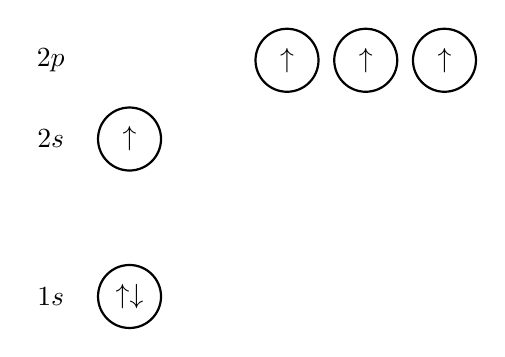
\begin{tikzpicture}[help lines/.style={thin,draw=black!50}] 
        %\draw[help lines] (0,0) grid (15,12);
        \foreach \x in {6,...,8} {
            \draw[thick] (\x,5) circle (0.4);
            \node at (\x,5) {$\uparrow$};
        }
        \draw[thick] (4,4) circle (0.4);
        \node at (4,4) {$\uparrow$};
        \draw[thick] (4,2) circle (0.4);
        \node at (4,2) {$\uparrow \downarrow$};
        \node at (3,5) {$2p$};
        \node at (3,4) {$2s$};
        \node at (3,2) {$1s$};
    \end{tikzpicture}
    \caption{Estado eletrônico do carbono que se obtém pela excitação de um elétron $2s$ ao orbital vazio $2p$.}
    \label{figura_2_8}
\end{figure}

 Embora não seja difícil perceber-se porque o carbono tende a ser tetravalente, é menos óbvio porque o carbono tende a formar compostos que são tetraedros regulares. Os quatro orbitais de valência da Figura \ref{figura_2_8} são três orbitais $p$, dispostos perpendicularmente uns aos outros, e um orbital $s$, esférico, e, portanto, sem direção definida. Uma ligação química é sempre mais forte quando os núcleos estão na linha de maior densidade eletrônica, de modo que esperaríamos, neste caso, que o átomo de carbono no metano estivesse no vértice de um cubo e três dos hidrogênios estivessem nos vértices a ele adjacentes, correspondendo às direções dos três orbitais $p$. Como o orbital $s$ é esférico, o quarto hidrogênio poderia estar em qualquer direção, como indicado na Figura \ref{figura_2_9}. Isto significaria que três dos ângulos seriam de 90$\degree$ e os demais não poderiam ser especificados. Esta estrutura não pode ser correta porque os quatro hidrogênios, como já vimos, têm de ser equivalentes. 

\begin{figure}[H]
    \centering
    \begin{tikzpicture}[help lines/.style={thin,draw=black!50}] 
        % \draw[help lines] (0,0) grid (15,12);
        \path (0,0) node (x) {H} (0,2) node (m) {C};
        \node (z) at ($ (m) + (20:2) $) {H};
        \node (y) at ($ (m) + (-3:2) $) {H};
        \draw[thick] (x) -- (m) -- (z);
        \draw[thick] (m) -- (y);
        % \node (b) at ($ (x) + (-3:2) $) {};
        \draw[dashed] (x) -- ($ (x) + (-3:2) $) -- (y) -- ($ (y) + (20:2) $) -- ++(-90:2) -- ++(200:2);
        \draw[dashed] (x) -- ($ (x) + (20:2) $) -- ++(-3:2);
        \draw[dashed] (z) -- ++(-90:2);
        \draw[dashed] (z) -- ++(-3:2);
        \draw[] (m) -- ++(90:2);
        \draw[] (m) -- ++(177:2);
        \draw[] (m) -- ++(200:2);
        \draw (-1,2.2) .. controls (-0.9,2.3) .. (-0.8,2.2) .. controls (-0.7,2.3) .. (-0.6,2.2);
        \node (H) at (-1.3,2.3) {H};
    \end{tikzpicture}
    \caption{Estrutura que esperaríamos para o metano se os orbitais de ligação não fossem hibridados.}
    \label{figura_2_9}
\end{figure}

A dificuldade aqui é teórica, uma vez que a evidência experimental é muito grande. O erro deve vir do fato de que estamos formando a ligação \ch{C—H} incorretamente. Os orbitais ($s$ e $p$) que usamos para descrever a molécula não estão corretos. Em outras palavras, o átomo de carbono deve ter sua descrição orbital alterada quando a ligação é feita. O sistema descrito no parágrafo precedente é uma solução aproximada satisfatória da equação Schrõdinger para a camada $n = 2$, mas podemos escrever combinações lineares dos quatro orbitais que são igualmente soluções da equação de Schrõdinger. (Os novos orbitais, obtidos dessas combinações lineares, são chamados de \textit{orbitais híbridos}.) Como construir \textit{orbitais híbridos} que satisfaçam as necessidades de geometria do tetraedro regular? A principal exigência é que os quatro orbitais devem ser equivalentes (de modo a formar quatro ligações \ch{C—H} equivalentes) e, portanto, a combinação linear adequada deve incluir os quatro orbitais de valência da Figura \ref{figura_2_8}. É matematicamente viável fazê-lo e os quatro novos orbitais terão caráter $\dfrac{1}{4} s$ e $\dfrac{3}{4}p$. Os quatro orbitais equivalentes contêm, portanto, três vezes mais caráter $p$ do que $s$ e são chamados orbitais $sp^3$.
\par\bigskip

\begin{leftbar}[cut=false]
\footnotesize

\noindent MATÉRIA OPCIONAL

\noindent \textit{Energética da hibridação}. Como uma ilustração específica, considere o átomo de neônio. A camada $n = 2$ está completa e a nuvem de elétrons total é esférica. (A densidade eletrônica total que resulta da existência de dois elétrons em cada orbital $2p$ é esférica, embora isto não seja aparente da inspeção das formas dos orbitais $p$.) Dois elétrons estão no orbital $2s$, com energia $E_8$ e seis elétrons estão nos orbitais $2p$, com energia $E_p$. A energia eletrônica total é, portanto $2E_8 + 6E_p$.

Se considerarmos quatro orbitais $sp^3$, cada qual com dois elétrons, a energia total é 8 elétrons $\times$ $(\dfrac{1}{4}E_8 + \dfrac{3}{4}E_p) = 2E_8 + 6E_p$, como acima, e os oito elétrons descrevem a mesma distribuição esférica. Assim, a descrição da camada externa do átomo de neônio pode ser feita igualmente em termos de um orbital $s$ e três orbitais $p$, ou em termos de quatro orbitais $sp^3$. Seria a mesma coisa que dizer que 12 é 3 $\times$ 4 ou 2 $\times$ 6. Ambas são corretas mas uma delas pode ser de uso mais conveniente. 

A hibridação dos orbitais não afeta a energia, distribuição eletrônica ou qualquer propriedade do estado fundamental do neônio, de modo que podemos utilizar ou não, a nossa escolha, orbitais híbridos. (Isto não é verdadeiro para estados excitados. Por quê?) 

Em um átomo de flúor, a distribuição eletrônica e a energia total dependem da hibridação e isto pode ser verificado usando-se sete elétrons e fazendo um cálculo semelhante ao que fizemos para o neônio. 
\end{leftbar}
\par\bigskip

Se examinarmos um mapa de contorno da densidade eletrônica de um orbital $sp^3$ veremos que apresenta dois lobos, como um orbital $p$, porém com tamanhos diferentes (Figura \ref{fig2_10}). Sabemos que para que se forme uma ligação forte é preciso que os elétrons de ligaçao possam permanecer entre os núcleos que se ligam. Um orbital $sp^3$, devido à sua forma, tem densidade eletrônica maior em uma direção especifica do que um orbital $s$ ou um orbital $p$ e, assim, devemos esperar que um orbital $sp^3$ possa formar uma ligação consideravelmente mais forte do que os orbitais $s$ ou $p$. Verifica-se, experimentalmente, que a força de uma ligação \ch{C—H} usando um híbrido $sp^3$ é de 103 kcal mol$^{-1}$, enquanto que com orbitais $s$ e $p$ e, respectivamente, de 60 e 80 kcal mol$^{-1}$. 

\begin{figure}[H]
    \centering
    \adjustbox{margin=1em,width=\textwidth,set height=4cm,set depth=4cm,frame,center}{Dummy}
    \caption{Mapa de contorno da densidade eletrônica do orbital $sp^3$.}
    \label{fig2_10}
\end{figure}

Mas toda essa discussão não teria sentido se não fosse pelo fato de que os quatro orbitais $sp^3$ guardam necessariamente entre si os ângulos de 109,5$\degree$, isto é, os ângulos internos do tetraedro regular. 

\begin{figure}[H]
    \centering
    \adjustbox{margin=1em,width=\textwidth,set height=4cm,set depth=4cm,frame,center}{Dummy}
    \caption{Densidade eletrônica em torno de um átomo de carbono com hibridação sp3. Mostramos apenas o maior lobo de cada orbital. Note que a densidade eletrônica total é esférica..}
    \label{fig2_11}
\end{figure}

Os orbitais híbridos $sp^3$ fornecem a melhor descrição do átomo de carbono no metano, porque o átomo de carbono (antes de formar a ligação) tem a mesma energia, hibridado ou não (Figura \ref{fig2_12}), mas a configuração hibridada permite formar ligações mais fortes. Há para a molécula de metano uma vantagem adicional na geometria tetraédrica. Tal arranjo permite o afastamento máximo dos núcleos de hidrogênio para uma dada distância \ch{C-H} e, uma vez que estes núcleos são carregados positivamente, quanto mais afastados os núcleos menor a energia do sistema.

\begin{figure}[H]
    \centering
    \adjustbox{margin=1em,width=\textwidth,set height=4cm,set depth=4cm,frame,center}{Dummy}
    \caption{Descrição eletrônica do carbono tetracovalente.}
    \label{fig2_12}
\end{figure}

Sumariando, o metano é tetraédrico e sua estrutura pode ser considerada como resultando da hibridação de quatro orbitais atômicos ($2s$, $2p_x$, $2p_y$ e $2p-z$), cada um contendo um elétron de valência, a quatro orbitais $sp^3$ equivalentes, os quais permitem a formação de ligações mais fortes e nas direções adequadas para minimizar as repulsões dos núcleos de hidrogênio. Assim, é possível descrever-se matematicamente as ligações da molécula de metano e entender-se o porquê de sua geometria. Melhor ainda, pode-se usar o conceito de orbitais híbridos para se entender moléculas mais complicadas (Seção 4.3). 

\par\bigskip
\noindent SOLUÇÃO DA EQUAÇÃO DE SCHRÖDINGER. \emph{Embora não seja possível a resolução da equação de Schrödinger, de maneira analítica, para moléculas contendo alguns átomos, é, em princípio, possível obter-se uma solução no grau de precisão desejado. Há mais ou menos 30 anos que sabemos como fazê-lo. Executar os cálculos complexos que são necessários é que é o problema. A solução tem de ser obtida usando-se métodos aproximados. Acontece que podemos expressar as propriedades de um átomo em termos de uma série infinita de orbitais e, para moléculas, combinações destas séries infinitas. Na prática reduzimos as séries a um número finito de termos maior ou menor, dependendo da precisão desejada na solução. Na resolução da equação de Schrödinger para uma molécula, é preciso multiplicar entre si muitas destas séries reduzidas, onde cada termo da multiplicação é uma integral de difícil avaliação. É evidente que a matemática envolvida torna o trabalho complicado. Após 1950, entretanto, grande progresso pôde ser feito nestes cálculos, graças ao desenvolvimento de computadores eletrônicos. O computador IBM 360/50, um típico computador de médio porte, de uso largamente difundido, pode executar 150.000 adições ou subtrações com sete algarismos significativos ou 50.000 multiplicações ou, ainda, 5.000 operações mais complexas (potências, raízes, funções trigonométricas) por segundo, com perfeição. Um problema de mecânica quântica pode necessitar de uma hora do tempo do computador e, sem qualquer dúvida, está fora da capacidade de um indivíduo que possua apenas uma régua de cálculo. A solução de problemas que seriam impossíveis em 1950 tornaram-se trabalho rotineiro. Por outro lado, soluções mais exatas para problemas comuns de moléculas poliatômicas (e para enfrentar o problema da reação química) exigirão computadores muito mais rápidos do que o IBM 360/50 (tão distantes em desempenho do IBM 360/50 do que este para as réguas de cálculo). De modo que, por enquanto, a teoria quântica é muito útil para dar respostas aproximadas aos mais diversos problemas da química, porém, exceto para moléculas pequenas, determinações precisas terão de ser feitas experimentalmente.}